% THIS IS SIGPROC-SP.TEX - VERSION 3.1
% WORKS WITH V3.2SP OF ACM_PROC_ARTICLE-SP.CLS
% APRIL 2009
%
% It is an example file showing how to use the 'acm_proc_article-sp.cls' V3.2SP
% LaTeX2e document class file for Conference Proceedings submissions.
% ----------------------------------------------------------------------------------------------------------------
% This .tex file (and associated .cls V3.2SP) *DOES NOT* produce:
%       1) The Permission Statement
%       2) The Conference (location) Info information
%       3) The Copyright Line with ACM data
%       4) Page numbering
% ---------------------------------------------------------------------------------------------------------------
% It is an example which *does* use the .bib file (from which the .bbl file
% is produced).
% REMEMBER HOWEVER: After having produced the .bbl file,
% and prior to final submission,
% you need to 'insert'  your .bbl file into your source .tex file so as to provide
% ONE 'self-contained' source file.
%
% Questions regarding SIGS should be sent to
% Adrienne Griscti ---> griscti@acm.org
%
% Questions/suggestions regarding the guidelines, .tex and .cls files, etc. to
% Gerald Murray ---> murray@hq.acm.org
%
% For tracking purposes - this is V3.1SP - APRIL 2009

\documentclass{acm_proc_article-sp}

\usepackage[hidelinks]{hyperref}
\usepackage{float}
\usepackage{subcaption}

\usepackage{listings}
\newcommand{\includecode}[2][C]{
    \lstinputlisting[breakatwhitespace=true, breaklines=true,
        basicstyle=\footnotesize, showstringspaces=false, 
        literate={"}{\textquotedbl}1, numbers=left, 
        language=#1]{#2}}

\floatstyle{boxed}
\newfloat{listing}{thp}{lop}
\floatname{listing}{Listing}

\begin{document}

\title{Implementation of Specialization Annotated OpenCL}

\numberofauthors{1}
\author{
\alignauthor
Nat Tuck\\
       \affaddr{University of Massachusetts Lowell}\\
       \affaddr{One University Avenue}\\
       \affaddr{Lowell, MA}\\
       \email{ntuck@cs.uml.edu}
}

\date{28 August 2014}

\maketitle

\begin{abstract}
This paper describes the implementation of Specialization Annotated OpenCL, an
extension to OpenCL to enable just in time value specialization. 

Value specialization, replacing a variable in a program with a known constant
for a particular data set, is an optimization that is commonly performed by
hand for HPC kernels. This optimization cannot be performed automatically in a
programming environment using ahead-of-time compilation, because the input data
is not available to the compiler. With OpenCL, kernel compilation is performed
just-in-time as the program runs, allowing the input data to be examined and
used during the compilation process.

We have developed an extension to OpenCL, Specialization Annotated OpenCL, that
allows some kernel arguments to be marked for specialization. This extension
has been implemented as a modification of POCL, an open source implementation
of OpenCL based on LLVM. Initial performance results on a multi-core CPU are
shown.

In addition, we have built a second implementation of Specialization Annotated
OpenCL as a library, suitable for use with proprietary implementations of OpenCL.
Initial performance results using this library are shown for AMD and Nvidia GPUs.
\end{abstract}

% A category with the (minimum) three required fields
\category{D.3.4}{Programming Languages}{Processors}[Compilers, Optimization, Just-In-Time]

\terms{Performance}

\section{Introduction}

When implementing an algorithm for an HPC application, it is a common practice
to embed specific values used in the computation in the program rather than
passing them in as parameters. For example, a program that simulated the
weather on a 500 meter grid may have the literal ``500 meters'' hard coded
as a global constant used throughout the program.

This technique has both advantages and drawbacks. As a non-HPC programmer, the
drawbacks are most obvious: hard coding a value makes changing the value more
difficult than if the value were passed as a parameter. Further, it means that
the code must be duplicated if the algorithm is used with two different values
in the same program execution. 

The advantage to hardcoding values is that the program will tend to run faster.
Compilers can do several optimizations with constant values that don't work as
well with variables, including arithmetic simplification and loop unrolling.

This technique is called value specialization. When a compiler does it, it is
sometimes called partial evaluation\cite{Futamura:1971:PE}.

It would be nice if the compiler could perform this optimization automatically
for values passed in to the program at run-time. Unfortunately, with traditional
ahead-of-time compilers this is impossible since run-time values are availble too
late for the compiler to use them.

OpenCL, the cross-platform parallel programming standard developed for GPU
programming, compiles compute kernels just-in-time as the program runs. We have
developed an exension to OpenCL, Specialization Annotated OpenCL, that allows
this optimization to be performed either by the compiler or by a library linked
in to an OpenCL program. Implementations using these two techniques are
described in Section~\ref{pocl-spec} and Section~\ref{pancake} respectively.

\section{Specialization Annotated OpenCL}

\begin{listing}
\includecode{mmul-spec.cl}
\caption{mmul.cl: Example specialization annotation}
\label{mmul-spec}
\end{listing}

\begin{listing}
\includecode{mmul-spec-example.cl}
\caption{mmul-codegen.cl: Execution model example.}
\label{mmul-spec-example}
\end{listing}

Specialization Annotated OpenCL extends OpenCL by adding annotations to mark
some arguments for specialization. Kernels are annotated by adding a specially
formatted comment as shown on the second line of Listing~\ref{mmul-spec}. This
comment comes between the argument list of the kernel and the opening brace of
the body and contains the {\tt @spec} symbol followed by the name of the kernel
and the list of arguments to be specialized in parentheses.

When a kernel with a specialization annotation is called, a specialized version
of that kernel is generated with the specialized arguments replaced by the values
used in that call. For example, if the kernel in Listing~\ref{mmul-spec} is called
with the values ($nn = mm = 8$), a specialized kernel is generated that is
functionally equvilent to the code shown in Listing~\ref{mmul-spec-example}.

Once the specialized kernel has been generated, it is called with the remaining
(non-specialized) arguments provided in the call. Specialized kernels are
cached for future calls with the same values for the specialized arguments.

\section{Specialization in POCL}
\label{pocl-spec}

POCL is an open source implementation of OpenCL supporting execution on
multi-core CPUs and several types of specialized acceleration hardware. It was
initially developed\cite{Jaaskelainen:2010:POCL} by Pekka Jaaskelainen and
others at the Tampere University of Technology in Finland and the Universidad
Rey Juan Calos in Spain in order to study the design of application specific
processor hardware, but has since been extended for use as a general purpose
OpenCL implementation. It is currently the most mature open source
implementation of OpenCL and provides good support for the OpenCL 1.2 standard
on x86\_64 multi-core CPUs.

POCL is built on the LLVM\cite{Lattner:2002:LLVM} compiler construction
toolkit. In broad strokes, POCL uses the
Clang\footnote{\url{http://clang.llvm.org}} C front end to parse OpenCL C and
generate LLVM IR, does most of its work in custom LLVM transformation passes,
and then uses an appropriate LLVM back-end to generate kernel binaries for
execution.

In order to extend POCL to support Specialization Annotated OpenCL, three
changes were needed. First, the OpenCL kernel source needed to be intercepted
to extract the specialization annotations. Second, the values of the
specialization variables needed to be extracted when the kernel was called.
Finally, an additional optimization pass needed to be added to during code
generation to perform the specialization.

\section{LLVM Specialization Pass}

In order to generate specialized kernels, an LLVM module
pass\cite{LLVM:Doc:WritePass} was written. This optimization pass operates by
iterating through the arguments of each kernel function in the module, seeing
if the name matches an argument marked for specialization in that kernel, and,
if so, replacing all uses of that argument's value with constant value
passed to the kernel call. 

The operation of replacing all uses of an argument with a new value is very
simple. The LLVM API provides a function ({\tt replaceAllUsesWith}) that does
exactly this. Because LLVM uses an SSA-based intermediate representation, this
works well even if the argument variable is modified during kernel execution,
which would be a problem if specialization was implemented by textual
substitution.

Specialization was implemented for 32-bit integers, 64-bit integers, floats,
and doubles. This was sufficent to run the various kernels used for testing the
implementation, but support for other scalar types could be easily added.
Specialization on arrays is an interesting possible extension (consider
specializing an image convolution function on a specific convolution matrix),
but this possibility was not explored.

\section{Performance}

In order to test the performance and correctness of the POCL-based
implementation of Specialization Annotated OpenCL, eight test cases were used
as described in Section~\ref{test-cases}. These tests were run on a 24-core
workstation with two AMD Opteron 6234 processors. The test machine had 32
gigabytes of RAM, which is well over the maximum required for any of the test
cases.

Each test case was run with six different compiler configurations, shown in
Table~\ref{test-configs}. The test cases were run five times for each
configuration. The results are shown in Figure~\ref{socl-pocl-table}. The bars
show the median measurement, while the error bars show minimum and maximum
measurements.

Initially, the main driver of performance gains was expected to be loop
unrolling enabled by making the loop trip count constant. This turned out not
to be the case. The Opteron's superscalar archetecture was 

% FIXME: Edit point here.

Four test cases showed
significant speedups, while two showed significant slowdowns. Loop unrolling
with specialization only provided a major benefit in two cases, when this was
expected to be the most significant mechanism for performance improvement.

The lower than expected benefit from loop unrolling caused in large part by cite{Jouppi:1989:ILP}. With multiple
arithmetic units and branch prediction it is able to optimize simple loops very
effectively in hardware.

Testing with processor with less instruction-level parallelism, the Atom N270,
confirmes this conclusion. Some tests got noticably greater benefit from
unrolling on this processor. Unfortunately, the Atom machine did not have
enough RAM to run the full set of test cases. Tests running on GPU devices also
showed similar results, as discussed in Section~\ref{gpu-tests}.

\begin{table}
\renewcommand{\arraystretch}{1.2}
\begin{tabular}{ l | p{2in} }
    {\bf default} & No optimizations \\
    \hline
    {\bf unroll} & Loop unrolling is enabled. \\
    \hline
    {\bf O3} & The full set of standard LLVM optimizations is enabled. \\
    \hline
    {\bf default-spec} & Specialization is enabled with no further optimizations. \\
    \hline
    {\bf unroll-spec} & Specialization and loop unrolling. \\
    \hline
    {\bf O3-spec} & Specialization and the full set of standard LLVM optimizations. \\
\end{tabular}
\caption{\label{test-configs} Compiler Configurations}
\end{table}

\begin{figure*}
\mbox{\hspace*{0.0\textwidth}
\begin{subfigure}[b]{0.55\textwidth}
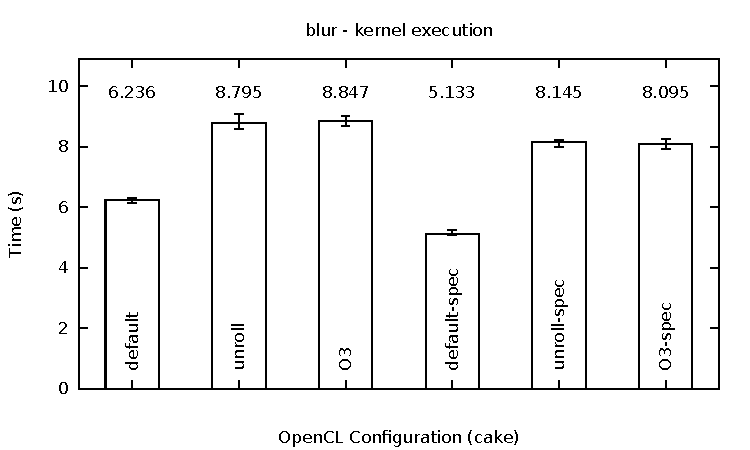
\includegraphics[width=3.0in]{charts/blur-exec}
\end{subfigure}
\begin{subfigure}[b]{0.55\textwidth}
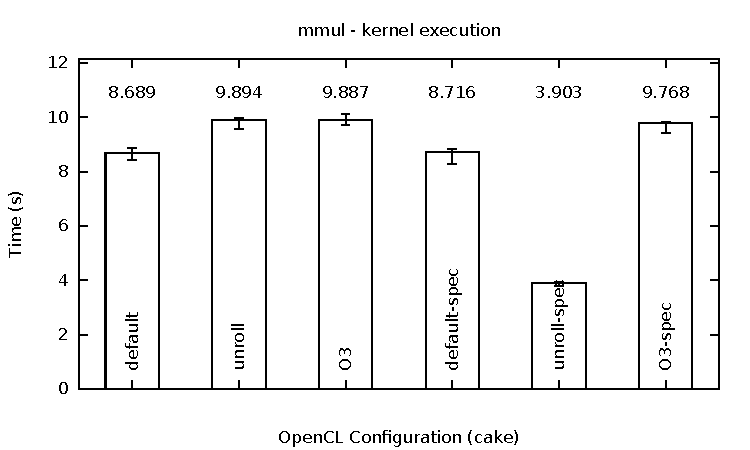
\includegraphics[width=3.0in]{charts/mmul-exec}
\end{subfigure}}

\mbox{\hspace*{0.0\textwidth}
\begin{subfigure}[b]{0.55\textwidth}
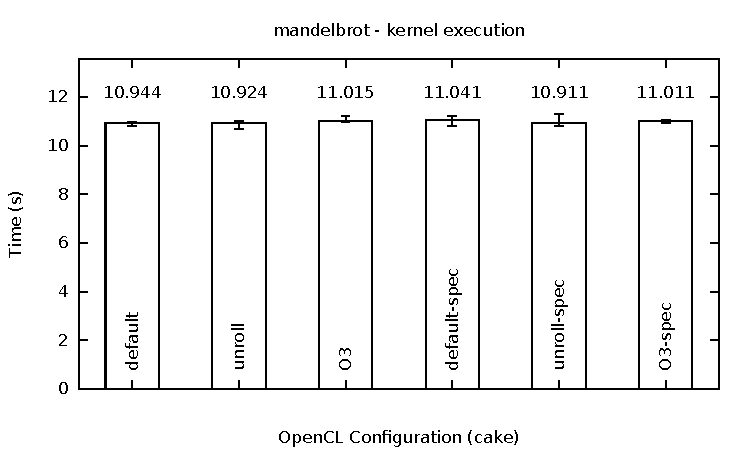
\includegraphics[width=3.0in]{charts/mandelbrot-exec}
\end{subfigure}
\begin{subfigure}[b]{0.55\textwidth}
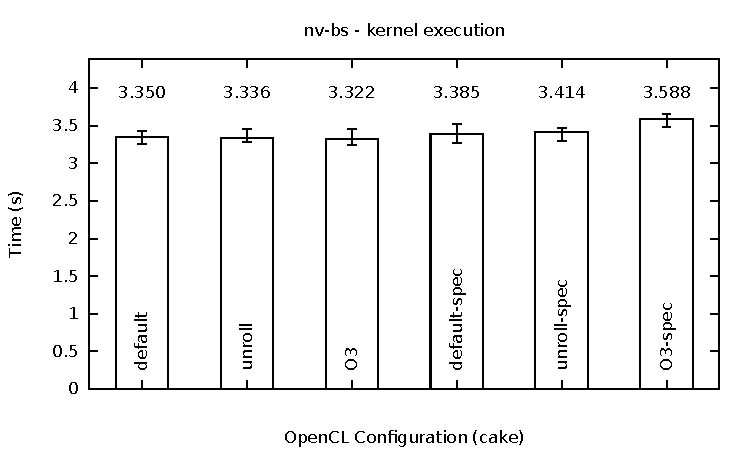
\includegraphics[width=3.0in]{charts/nv-bs-exec}
\end{subfigure}}

\mbox{\hspace*{0.0\textwidth}
\begin{subfigure}[b]{0.55\textwidth}
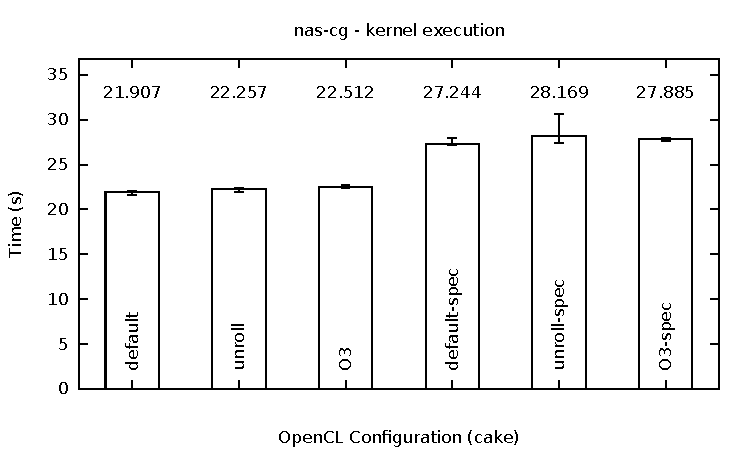
\includegraphics[width=3.0in]{charts/nas-cg-exec}
\end{subfigure}
\begin{subfigure}[b]{0.55\textwidth}
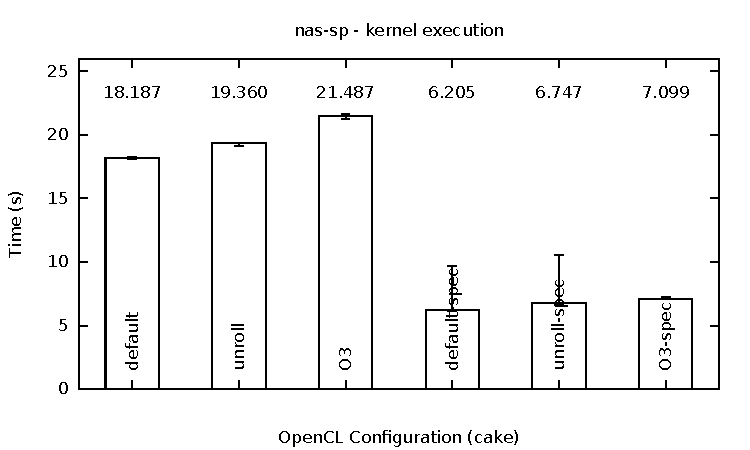
\includegraphics[width=3.0in]{charts/nas-sp-exec}
\end{subfigure}}

\mbox{\hspace*{0.0\textwidth}
\begin{subfigure}[b]{0.55\textwidth}
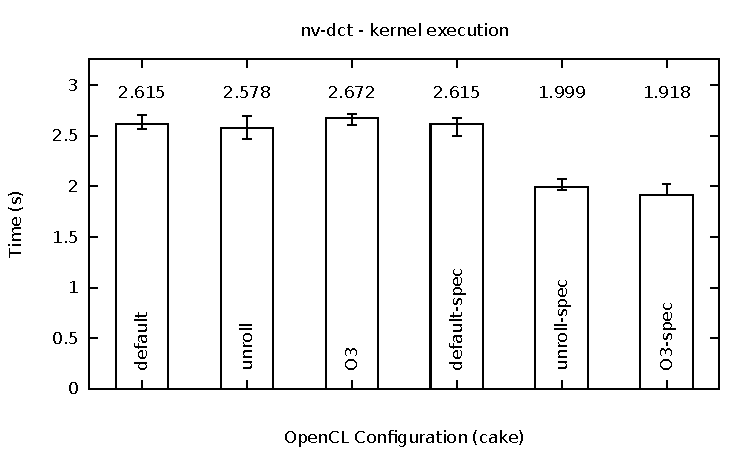
\includegraphics[width=3.0in]{charts/nv-dct-exec}
\end{subfigure}
\begin{subfigure}[b]{0.55\textwidth}
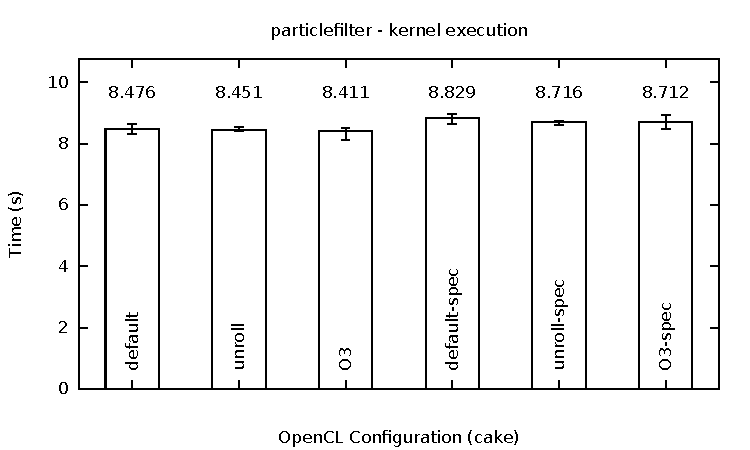
\includegraphics[width=3.0in]{charts/particlefilter-exec}
\end{subfigure}}

\caption{\label{socl-pocl-table} Benchmark Timings for Specialization Annotated OpenCL}
\end{figure*}

\section{Test Cases}
\label{test-cases}

In order to test the implementation of Specialization Annotated OpenCL, eight
OpenCL programs were selected and annotated for specialization. Two of these
test cases are newly written, while the other six were taken from existing
OpenCL benchmarks and vendor sample code.

\subsection{Newly Written Test Cases}

These programs were written specifically as test cases for this project. They
are intentionally written as naive implementations of the algorithm, without
any hand optimization. This may make performance effects from optimization
easier to see compared to the highly optimized test programs taken from
hardware benchmark suites.

\subsubsection{Gaussian Blur (blur)}

This program applies Gaussian blur to a large (5184x3456) greyscale image.
Because a 2D Gaussian blur can be calculated by applying two orthogonal 1D
Gaussian blurs to an image in sequence, this program runs two OpenCL kernels:
one to blur vertically and one to blur horizontally.

The kernels are each specialized on three arguments, the width and height of
the image and the radius of the blur effect. The radius is used for the inner
count of a tight inner loop, so its specialization was expected to result in a
measurable performance benefit due to unrolling.

The best speedup on this test was 22\%, with no optimizations.

\subsubsection{Matrix Multiply (mmul)}

This program multiplies two square matrices. Although matrix multiply programs
are common in OpenCL vendor samples, they are generally optimized to take
advantages of features like vector types. This program was written specifically
to be a simple and easily readable version of parallel matrix multiply.

The kernel is specialized on two arguments: the width and height of the
matrices. Since the iteration count of the inner loop is dependent on the width
and height of the matrices, this test should show measurable performance
improvement from specialization.

\subsection{SNU Port of NAS Parallel Benchmarks}

This is a port of the NASA Advanced Supercomputing Division's NAS Parallel
Benchmark\cite{Van:2002:NAS} suite for large parallel HPC installations to
OpenCL, performed by the Center for Manycore Programming at Seoul National
University in Korea\cite{Seo:2011:NASPerf}.

These benchmarks are reasonably complex and require a significant amount of
communication in patterns that are not easily implemented in OpenCL, so the SNU
developers put significant effort into splitting kernels for synchronization
and hand optimizing to get high speedups.

\subsubsection{Conjugate Gradient (nas-cg)}

This program is described by the NAS benchmark description as ``Solving an
unstructured sparse linear system by the conjugate gradient method'' with the
benchmark goal of testing ``irregular memory access and communication''.

For the OpenCL implementation this program was split into 13 kernels. The kernels
were all specialized on a single argument, {\tt n}, which remains constant across
any single execution of the program. As this argument is not used directly as
the bound of any loop, specialization and loop unrolling seem unlikely to provide
any performance benefit.

\subsubsection{Scalar Penta-Diagonal (nas-sp)}

This program is intended to represent a larger HPC application that involves
multi-step processing of data. It performs a fluid dynamics simulation.

This program uses 26 OpenCL kernels. Fourteen of these kernels are specialized
on parameters that stay nearly constant in a single execution of the program,
some of which are used as loop bounds. This program may see benefits from
specialization.

\subsection{Nvidia OpenCL Samples}

These program were released by Nvidia as sample programs to demonstrate the
usage of their OpenCL implementation. They are written primarily for clarity to
serve as good examples, but include some features intended to improve
performance.

\subsubsection{Black-Scholes Option Pricing (nv-bs)}

According to Nvidia, ``This sample evaluates fair call and put prices for a
given set of European options by the Black-Scholes formula.'' 

This kernel is specialized on a single variable, {\tt OptN}, which is the maximum
number of iterations of the algorithm. This is a constant across multiple calls
to the kernel in the test program. It specifies the iteration limit of a
reasonably tight inner loop, but the loop start varies across work items so the
loop may not be possible to unroll. Specialization may or may not provide a
performance benefit on this program.

\subsubsection{DCT (nv-dct)}

This program performs a Discrete Cosine Transform on an image.

The kernel is specialized on the stride, width, and height of the input image,
and the block size of the transform, which all remain constant in the test
program. The program was initially developed with a constant block size of
eight, but this was made a variable in order to exercise specialization. Since
all the loops in the program are a number of iterations equal to the block size,
this program should see speedups due to specialization.

\subsection{Rodinia Benchmarks}

These benchmarks were found in the Rodinia Benchmark
Suite\cite{Rodinia:Benchmarks}, from the University of Virginia. This suite is
intended to compare the performance of hardware and OpenCL implementations.
The benchmarks are extracted from real world scientific computing applications,
and are heavily hand optimized for performance.

\subsubsection{Mandelbrot (mandelbrot)}

This generates a 2048x2048 image of the Mandelbrot set. It has a single OpenCL
kernel to generate this image.

The kernel is specialized on four arguments: the width and height of the image,
the zoom level, and the maximum number of iterations of the tight inner loop.
Although the number of iterations of the tight inner loop is bounded by a
specialized argument, each instance of the kernel may iterate less times.
Specialization may not provide a significant performance advantage in this test
if the loop cannot be unrolled.

\subsubsection{Particle Filter (particlefilter)}

This program tries to estimate current location based on a model of movement
and fuzzy location measurements. 

The main kernel is specialized on the number of particles used, which is
constant through an execution of the program. This kernel has a loop based on
the number of particles, but the start point is based on the current particle
so the loop may not be possible to unroll. This program may or may not see
speedups from specialization.



\bibliographystyle{abbrv}
\bibliography{references}

\balancecolumns

\end{document}
